Error propagation in a text processing chain is usually a notable problem, therefore accurate segmentation methods are essential to parse texts properly.
Moreover, notes written by doctors are extremely noisy containing errors which inhibit the application of existing tools.

Even though tokenization and sentence segmentation methods perform well on general Hungarian, they have serious difficulties on clinical records.
These originate in special properties of such texts involving
\begin{enumerate} %[\itshape a\upshape)]
 \item typing errors (i.e. mistyped tokens, nonexistent strings of falsely concatenated words) and
 \item nonstandard usage of the language.
\end{enumerate}
While errors of the first type can be corrected easily with a rule-based tool, others need advanced methods. 

In this section, a hybrid approach to segmentation of noisy clinical records is presented. 
The method consists of two phases: first, tokens are partially segmented; then, sentence boundaries are identified.
We start with detailing the background of our research and introducing resources used.
Then, key elements of tokenization and \gls{sbd} algorithms are described. 
Finally, our system is systematically evaluated on a gold standard corpus showing its high performance.

\subsection{Previous approaches on text segmentation}

Even though, numerous studies deal with English medical texts, only few attempts have been made (cf. \cite{Siklosi2012,Siklosi2013,Siklosi2013b}) for Hungarian. 
Further on, the task of detecting sentence and word boundaries in health records is often a neglected issue.
Studies for Hungarian pay almost no attention on segmenting texts, while
most of the approaches for English ignore this question. 
First, we review general tokenization and sentence boundary detection techniques first, then describe their application on the biomedical domain.

The task is often composed of several parts: normalization (when necessary), tokenization, and sentence boundary detection.  
Although, these are generally performed one after another, there are approaches (e.g. \cite{zhu2007unified}), where tokenization and \acrshort{sbd} are treated as a unified tagging problem (such as in \cite{mikheev2000tagging}). 
Further on, handling of abbreviations is often involved in the segmentation process, since their identification helps to detect sentence and token boundaries.

As regards tokenization, it is generally treated as a simple engineering problem\footnote{In the case of alphabetic writing systems.} cutting off punctuation marks from words. 
On the contrary, \acrshort{sbd} is a rather researched topic. 
As Read et al. summarize \cite{read2012sentence}, sentence segmentation approaches fall into three classes: 
\begin{enumerate}
 \item rule-based methods employing domain- or language-specific knowledge (such as abbreviations); 
 \item supervised machine learning approaches, which may not be robust amongst domains (being specialist on the training corpus); and
 \item unsupervised learning methods extracting their knowledge from raw unannotated data. 
\end{enumerate}

As regards \acrshort{ml} attempts, one of the first pioneers was Riley \cite{riley1989some} who employed decision-tree learners to classify full stops. 
He utilized mainly lexical features (such as word length or case) to compute the probability of a word being sentence-initial or sentence-final. 
Next, Palmer et al. presented \cite{palmer1997adaptive} the SATZ system, employing supervised learning algorithms. 
Since this tool can be easily adjusted through surface and syntactic features, it has been successfully applied to several European languages. 
Further on, the maximum entropy learning approach was used as well to the task by Reynar and Ratnaparkhi \cite{reynar1997maximum}. 
Their system classifies tokens containing `.', `?' or `!' characters utilizing contextual features and abbreviation lists. 
Recently, a similar approach has been presented by Gillick \cite{gillick2009sentence} for English, using applying vector machines and resulting in state-of-the-art performance.

Beside machine learning approaches, rule-based methods are also commonly applied for these tasks. 
E.g. Mikheev presents \cite{mikheev2002periods} a small set of rules for detecting sentence boundaries (\acrshort{sb}) with a high accuracy. 
In another system presented of him \cite{mikheev2000tagging}, the latter method is integrated into a \acrshort{pos} tagging framework enabling the classification of punctuation marks. 
In doing so, they can be labeled as sentence boundaries, abbreviations or both. 
Moving on, Kiss and Strunk have introduced \cite{kiss2006unsupervised} an unsupervised method for sentence boundary detection in 2009. 
Their tool, Punkt uses scaled log-likelihood ratio for deciding whether a \emph{(word, full stop)} pair is a collocation or not.

Although tokenization and \acrshort{sbd} tasks are well established fields of natural language processing, there are only a few attempts aiming medical texts. 
These sentence segmentation attempts fall into two classes: some develop rule-based systems (e.g. \cite{XuSDJWD10}), while most of the studies employ supervised machine learning algorithms (such as \cite{apostolova2009automatic,cho2002text,Savova2010,taira2001automatic,tomanek2007sentence}).
Latter approaches usually train \acrlong{maxent} or \acrshort{crf} learners, thus large handcrafted training corpora are essential. 

Training data used are either domain-specific or general. 
In practice, domain-specific knowledge yield better performance, however Tomanek et al.  \cite{tomanek2006reappraisal} argue on using only a general-purpose corpus. 
Their results indicate that the domain of the training corpus is not critical (at least for German).

As regards Hungarian, there are only two tools available. 
Huntoken \cite{Halacsy2004} is an open source system based on Mikheev’s system, while \texttt{magyarlanc} \cite{zsibrata2013magyarlanc} has an adapted version of MorphAdorner’s rule-based tokenizer \cite{kumar2009monk} and sentence splitter. 
Both of them employ general-purpose methods utilizing language- and domain-specific rules and dictionaries.

This study introduces new methods for segmenting Hungarian clinical texts.
For this, special properties of the target domain is investigated first by creating a manually segmented corpus. 
Then, a method is presented which combines high precision rules with unsupervised learning.

\subsection{Evaluation metrics}
\label{sec:metric}

There is no metric commonly used to measure segmentation methods, therefore we review existing ones.
On the one hand, researchers specializing in machine learning approaches prefer to calculate precision, recall and $F$-measure. 
However, these scores are often used for measuring the correctness of sentence boundaries only.
On the other hand, studies on speech recognition prefer to compute NIST and Word Error Rate. 

Recently, Read et al. have reviewed \cite{read2012sentence} the state-of-the-art of text segmentation proposing a unified metric to compare different approaches. 
Their method allows measuring sentence boundaries at any position labeling characters as sentence-finals or non sentence-finals. 
In doing so, simple accuracy measures the performance. 

Our study builds on their results \cite{read2012sentence} adapting it to the full segmentation task of Hungarian clinical texts. 
In that way, we consider the corpus as a sequence of characters and empty strings and treat text segmentation as a single classification problem. 
Therefore, all the entities (either characters or empty string between them) can be labeled with one of the following tags: 
\begin{description}
 \item[$\langle$T$\rangle$] --  if the entity is a token boundary,
 \item[$\langle$S$\rangle$] -- if it is a sentence boundary,
 \item[$\langle$None$\rangle$] -- otherwise.
\end{description}
This classification scheme enables us to compute accuracy of the unified segmentation task. 
Moreover, it allows computing further common metrics.

Since it is important to measure each subsystem's correctness, precision and recall were computed for both word tokenization and \acrlong{sbd}. 
Further on, word segmentation was evaluated with $F_1$, while $F_{0.5}$ was computed for the \acrshort{sbd} task. 
(The latter calculation makes precision more important than recall.)
We employed the latter metric, because an erroneously split sentence may cause information loss\label{sec:loss}, while statements might still be extracted from longer multi-sentence text. 

\subsection{Clinical texts used}
\label{sec:clin_corpus}

A gold standard corpus of clinical texts was collected and manually corrected in order to develop and evaluate segmentation approaches.
This process involved several steps involving normalization, as such texts are full with diverse mistakes. 
In doing so, we had to deal with the following types of errors\footnote{Text normalization steps were carried out employing regular expressions.}:
\begin{enumerate}
 \item doubly converted characters, such as `\&amp;gt;',
 \item typewriter problems (e.g. `1' and `0' is written as `l' and `o'),
 \item dates and date intervals being in various formats with or without necessary whitespaces (e.g. `2009.11.11', `06.01.08'),
 \item missing whitespaces between tokens usually introduced various types of errors, such as:
 \begin{enumerate}
  \item measurements were erroneously attached to quantities (e.g. `0.12mg'),
  \item lack of whitespace around punctuation marks (e.g. `töröközegek.Fundus:ép.'),
 \end{enumerate}
 \item various formulation of numerical expressions.
\end{enumerate}
 
To investigate possible pitfalls, the gold standard data is split into two parts of equal sizes: a development and a test set containing 1,320 and 1,310 sentences respectively. 
The first part was used to identify typical problems and to develop the segmentation methods, while the second one was employed to evaluate the results. 

As initial step, the distributions of abbreviations, punctuation marks and capitalization is investigated in these texts to reveal possible difficulties. 
Comparing our data with a corpus of general Hungarian (Szeged Corpus \cite{Csendes2004}) uncovers numerous discrepancies: 
\begin{enumerate}
 \item 2.68\% of tokens found in clinical corpus sample are abbreviations while the same ratio for general Hungarian is only 0.23\%; 
 \item sentences taken from the Szeged Corpus almost always end in a sentence final punctuation mark (98.96\%), while these are totally missing from clinical statements in 48.28\% of the cases; 
 \item sentence-initial capitalization is a general rule in Hungarian (99.58\% of the sentences are formulated properly in the Szeged Corpus), but its usage is not common in the case of clinicians (12.81\% of the sentences start with a word that is not capitalized); 
 \item the amount of numerical data is notable in medical records (13.50\% of sentences consist exclusively of measurement data and abbreviations), while text taken from the general domain rarely contains statements that are full of measurements. 
\end{enumerate}

%Concidering that general-purpose tools may have difficulties with texts from this domain. 
%Such methods usually builds on features such as word capitalization and presence of punctuation marks, however their usage is significantly differ in our case. 



\subsection{Segmentation methods}
\label{sec:clinical_segmentation}

Our system is built up from several components (cf. Figure \ref{fig:clin-segment-arch}). 
First, a symbolic method (referred as the baseline) marks word and sentence boundaries\footnote{Rules and heuristics used are formulated investigating the development corpus.} seeking for full stops. 
Then, an unsupervised filtering method extends its output.
Finally, rules employing capitalization yields further sentence boundaries.

\begin{figure}[H]
  \centering
  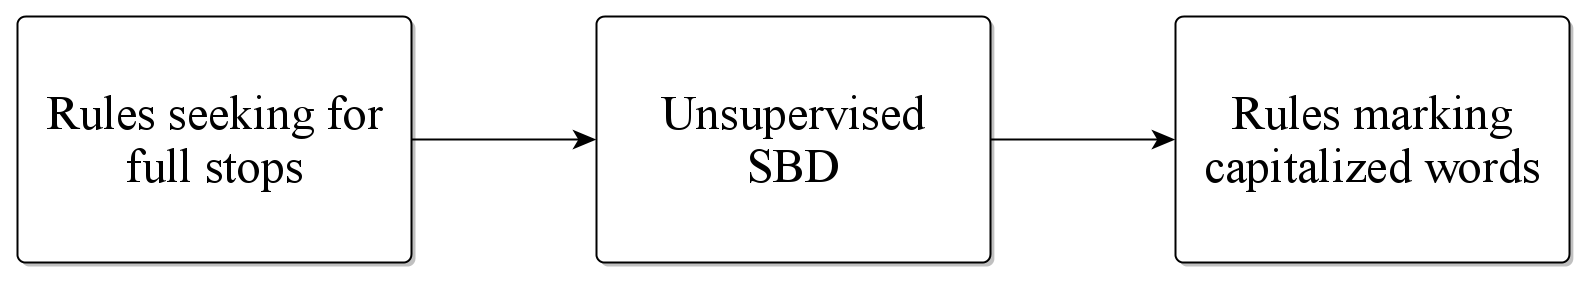
\includegraphics[scale=0.2]{Clinical/clin_segm_arch.png} 
  \caption{The architecture of the proposed method}
  \label{fig:clin-segment-arch}
\end{figure}

\subsubsection{Rule-based word tokenization and sentence segmentation}

Our baseline method is composed of two parts. 
First, it tokenizes words (BWT) using regular expressions implemented in standard tokenizers. %then some of the sentence boundaries are classified.
However, this algorithm does not try disambiguate all words containing periods, as it would need the proper recognition of domain-specific abbreviations as well. %Therefore it only marks just a few boundaries

Further on, sentence segmentation (BSBD) is carried out minimizing information loss (as described in section \ref{sec:loss}). 
In that way, the method tries to avoid of making false-positive errors by splitting sentences only if there is a high confidence of success. 
We found that such cases are, when:
\begin{enumerate} 
 \item a period or exclamation mark directly follows another punctuation mark\footnote{Question marks are not considered as sentence-final punctuation marks, since they generally indicate a questionable finding in clinical texts.};
 \item a line starts with a full date, and is followed by other words (The last white-space character before the date is marked as a \gls{sb}.);
 \item a line begins with the name of an examination followed by a semicolon and a sequence of measurements.
\end{enumerate}

Realization of these simple observations yield 100\% precision and 73.38\% recall on tokenization considering the development set. 
The corresponding values for detecting ends of sentences are 98.48\% and 42.60\% respectively. 
As less than half of the sentence boundaries are discovered, this method needs further improvements.
In addition, a deeper analysis unfolded that the tokenization module has difficulties only with sentence final periods. 
We found that these sorts of errors are effects of the conservative tokenization algorithm, which left several words with punctuation mark attached ambiguous.
%In that way, the algorithm is adjusted incorporating unsupervised learning.

%\subsubsection{Improvements on sentence boundary detection}\label{sec:improvements}
\subsubsection{Unsupervised sentence boundary classification}

In order to enhance the baseline method we considered investigating two kinds of indicators that are usually employed in such scenarios:
%There are two indicators generally used for detecting sentence boundaries.
\begin{description}
 \item[Periods:] when a punctuation mark ($\bullet$) is attached to a word, a sentence boundary is found for sure only if the token is not an abbreviation.
 \item[Capitalization:] if a word starts with a capital letter and it is neither part of a proper name nor of an acronym, it indicates the beginning of a sentence.
\end{description}
Considering our case:
\begin{enumerate}
\item clinicians introduce new abbreviations frequently which are not part of the standard, therefore a proper list cannot be collected easily, further on, 
\item Latin words, abbreviations and subclauses are sometimes capitalized by mistake, thus they are neither reliable information sources.
\end{enumerate}
In addition, numerous sentence boundaries lack both of these indicators (as shown in Section \ref{sec:clin_corpus}). %Therefore, these are not directly applicable in our case. 

Even though these features do not function regularly, they can still be utilized.  %without a list of possible abbreviations. 
It is enough to find \emph{evidence} for the separateness of a word and the subsequent full stop to classify a position as a sentence boundary. 
For this, we employed the idea of Kiss and Strunk \cite{kiss2006unsupervised} and adapted it for clinical texts.

Their method (log-likelihood ratio) was first applied to identify collocations \cite{dunning1993accurate}, however, they managed to adjust it for the \acrshort{sbd} problem recently (cf. Punkt\cite{kiss2006unsupervised}). 
The Punkt tool considers abbreviations as collocations of words and periods, thus evaluating them using a modified log-likelihood ratio.
In practice, this is formulated via a null hypothesis \eqref{eq:h0} and an alternative one \eqref{eq:ha}. 

\begin{equation} \label{eq:h0}
H_0: P(\bullet|w) = p = P(\bullet|\neg w)
\end{equation}

\begin{equation} \label{eq:ha}
H_A: P(\bullet|w) = p_1 \neq p_2 = P(\bullet|\neg w) 
\end{equation}

\begin{equation} \label{eq:loglambda}
\log \lambda = -2 \log \frac{L(H_0)}{L(H_A)}
\end{equation}


In these formulae, $H_0$ expresses the independence of a \emph{(word, $\bullet$)} pair, $H_1$ formulates that their co-occurrence is not just by chance, while $L$ denotes the likelihood function. 
The log-likelihood ratio of the null and alternative hypothesis is measured by the $\log \lambda$ score \eqref{eq:loglambda}, which is found to be asymptotical to $\chi^2$ \cite{dunning1993accurate}. %, thus  can be applied as a statistical test \cite{dunning1993accurate}. 
However, Kiss and Strunk recovered that this simple method performs poorly (in terms of precision) for identifying abbreviation.
Therefore, they adapted the likelihood-ratio test by introducing several factors for scaling its result \cite{kiss2006unsupervised}, and transforming it a heuristic ranking algorithm.

We improved their approach in numerous ways. 
First of all, the inverse score ($iscore=1/log\lambda$) was used as a base, since it helps to find candidates co-occurring only by chance. 
Moving on, we introduced further scaling factors reviewing that of Punkt and adapting them to match the characteristics of the target domain.

First of all, the first factor of the Punkt system cannot be directly applied in our case.
Counts and count ratios alone do not indicate properly alone whether a token and the period is related in a clinical record, since several sorts of abbreviations occur with relative low frequencies. 


Next, lengths of words ($len$) was also used in Punkt to indicate abbreviations well. 
They could help in our case, since shorter tokens tend to be abbreviations, while longer ones do not. 
Therefore, we reformulated the original function to penalize short words and reward longer ones. 
Having a medical abbreviation list of almost 200 \label{sec:abbrev} elements\footnote{The list is gathered with an automatic algorithm on the development corpus using word shape properties and frequencies. The most frequent elements are manually verified and corrected.} 
we found that more than 90\% of the abbreviations are shorter than three characters. 
This fact led us to formulate the scaling factor as in \eqref{eq:s_l}. 
In doing so, this enhancement can also decrease the score of a bad candidate, which distinguishes it from the original formula of Kiss and Strunk.

\begin{equation} \label{eq:s_l}
S_{length}(iscore)= iscore \cdot \exp{(len/3-1)}
\end{equation}

Recently, Humor ~\cite{Proszeky1994,Novak2003,Proszeky2005}  has been extended with the content of a medical dictionary \cite{Orosz2013}. 
What is more, the analyzer is able indicate whether analyses refers to abbreviations.
Therefore, its output is used to enhance the sentence segmentation algorithm.  

An indicator function was introduced (cf. Equation \ref{eq:sign}) to utilize its output deciding whether a word can be an abbreviation or not.
Since, the morphological lexicon used is a well-established resource, our application could rely on it with high confidence.
Therefore, the factor formulated (cf. Equation \ref{eq:s_m}) uses larger weights compared to others. 
This method raises the score of a full word, decreases that of an abbreviation, while values of unknown words are left as they were.

\begin{equation}\label{eq:sign}
 indicator_{morph}(word) =
  \begin{cases}
   1  & \text{if $word$ has an analysis of a known full word} \\
   -1 & \text{if $word$ has an analysis of a known abbreviation} \\
   0  & \text{otherwise}
  \end{cases}
\end{equation}

\begin{equation} \label{eq:s_m}
S_{morph}(iscore)= iscore \cdot \exp{( indicator_{morph} \cdot len^2)}
\end{equation}

%Besides, utilization of an additional attribute of tokens can also boost the segmentation process.
Hyphens are generally not present in abbreviations but rather occurs in full words. 
Relying on this observation, $iscore$ was adjusted \eqref{eq:s_h} with a further indicator function:
$indicator_{hyphen}$ outputs $1$ only if the word contains a hyphen. 

\begin{equation} \label{eq:s_h}
S_{hyphen}(iscore)= iscore \cdot \exp{(indicator_{hyphen} \cdot len)}
\end{equation}

\begin{equation} \label{eq:scaling}
S = S_{length} \circ S_{morph} \circ S_{hyphen}
\end{equation}

Scaled $\log \lambda$ (cf. $S(iscore)$ in Equation \ref{eq:scaling}) is calculated for all \emph{(word, $\bullet$)} pairs not followed by any other punctuation mark. 
If this value is found to be higher than a threshold, the period is regarded as a sentence boundary and it is detached.\footnote{Threshold value is empirically set to $1.5$.} 
Otherwise, the joint token is treated as an abbreviation.

To investigate the improvement of our method, it was pipelined with the BSBD module producing 77.14\% recall and 97.10\% precision on the development set. 
Accuracy values show significant improvements, however they also indicate that many sentence boundaries are still not found.

\subsubsection{Rules on capitalization}

To further improve the method, capitalization properties of words were also utilized. 
We developed a rule-based component to decide whether a capitalized words can start a sentence or not.
Good \acrshort{sb} candidates of such tokens are the ones not following a non sentence terminating\footnote{Sentence terminating punctuation marks are the period and the exclamation mark for this task.} punctuation, and are not part of a named entity. 
Therefore, sequences of capitalized words are considered to be named entities and omitted as a first step. 
Then, the rest of the candidates are processed by Humor.
We employed a simple heuristic for detecting sentence boundaries:
if a word does not have a proper noun analysis but is capitalized, it is marked as the beginning of a sentence.  
Our results on the development set show that this component also enhances the BSBD: it increases recall to 65.46\% while keeps precision high (96.37\%). 

\subsection{Evaluation}

% Our hybrid algorithm has been developed using the development set, thus it is evaluated against the rest of the data. 
% %As the starting point of our comparison, we present the accuracy values of the preprocessed input text and the baseline tokenized one. 

\begin{table}[H]
\centering
\caption{Accuracy of the input text compared with segmented ones}
\label{tab:base}
\begin{tabular}{ l  r } 
\hline
& Accuracy \\ 
\hline
Raw corpus  & 97.55\% \\
BSBD & 99.11\% \\
\hspace{0.2cm}+ LLR & 99.72\% \\
\hspace{0.2cm}+ CAP & 99.26\% \\
\hspace{0.2cm}+ LLR + CAP & 99.74\% \\
\hline
\end{tabular}
\end{table}

Evaluation is presented for each components showing their accuracies (cf. Table \ref{tab:base}).
First, our improvements are compared to both the baseline module and the raw preprocessed corpus.
The unsupervised \acrshort{sbd} algorithm is marked with LLR\footnote{Referring to the term log-likelihood ratio.}, while the last component is indicated by CAP.
Results show high accuracies for the overall segmentation task, furthermore the scores of the raw corpus is relatively high.
This indicates that the metric applied is not well balanced.

Therefore, their improvements are also investigated calculating \acrlong{err} ratios (in Table \ref{tab:reduction}). 
Comparison is carried out measuring enhancements over the baseline method (BSBD) showing that both of the components improves the segmentation method.

\begin{table}[H]
\centering
\caption{Error rate reduction over the baseline method}
\label{tab:reduction}
\begin{tabular}{ l  r } 
\hline
& Error rate reduction\\
\hline
LLR & 58.62\% \\
CAP & 9.25\% \\
LLR + CAP & 65.50\% \\
\hline
\end{tabular}
\end{table}

Considering sentence boundaries only, a more detailed analysis is got by computing precision, recall and $F_{0.5}$ values (in Table \ref{tab:prec_rec}). 
Data shows that each component significantly increases the recall, while precision is just barely decreased. 
Finally, the combined hybrid algorithm\footnote{It is the composition of the BWT, BSBD, LLR and CAP components.} brings significant improvement over the well-established baseline.

\begin{table}[H]
\centering
\caption{Evaluation of the proposed sentence segmentation algorithm compared with the baseline}
\label{tab:prec_rec}
\begin{tabular}{ l r r  r  } 
\hline
& Precision & Recall & $F_{0.5}$ \\
\hline
Baseline & 96.57\% & 50.26\% & 81.54\%  \\
+ LLR & 95.19\% & 78.19\% & 91.22\% \\
+ CAP & 94.60\% & 71.56\% & 88.88\% \\
+ LLR + CAP & 93.28\% & 86.73\% & \underline{91.89\%} \\
\hline
\end{tabular}
\end{table}


While our approach focuses on the sentence identification task, we showed that it improves word tokenization as well. 
Table \ref{tab:tok_eval} presents measurements on word segmentation indicating that our enhancements resulted in a higher recall, while they did not decrease precision notably. \label{sec:eval}

%0.9974	0.7494	0.8558
%0.9854	0.9532	0.9690
%0.9974	0.7494	0.8558
%0.9854	0.9532	0.9690

\begin{table}[H]
\centering
\caption{Comparing tokenization performance of the new tool with the baseline one}
\label{tab:tok_eval}
\begin{tabular}{ l r r r} 
\hline
& Precision & Recall & $F_{1}$ \\
\hline
Baseline & 99.74\% & 74.94\% & 85.58\%  \\
Hybrid system & 98.54\% & 95.32\% & \underline{96.90\%} \\
\hline
\end{tabular}
\end{table}

Besides, the proposed method was compared with freely available tools as well (
%There are only two applications for Hungarian text segmentation: 
\texttt{magyarlanc} and Huntoken)
The latter system can be slightly adapted to a new domain by providing a set of abbreviations, thus two versions of it were evaluated. 
The first one employs a set of general Hungarian abbreviations (HTG), while the second one utilizes an extended dictionary\footnote{As described in section \ref{sec:abbrev}.} containing medical ones as well (HTM). 
Further on, Punkt \cite{kiss2006unsupervised} and the OpenNLP \cite{Baldridge2002} toolkit\footnote{The general-purpose Szeged Corpus was used as training data for the \acrlong{maxent} learning method.} were also involved in our comparison. 
The latter tool is a general framework of \acrlong{maxent} methods, hence it could be applied to detect sentence boundaries as it is presented in \cite{reynar1997maximum}.


\begin{table}[H]
\centering
\caption{Comparison of the proposed hybrid \acrshort{sbd} method with competing ones}
\label{tab:comparison}
\begin{tabular}{ l r r r} 
\hline
& Precision & Recall & $F_{0.5}$ \\
\hline
\texttt{magyarlanc} & 72.59\% & 77.68\% & 73.55\% \\
HTG & 44.73\% & 49.23\% & 45.56\% \\
HTM & 43.19\% & 42.09\% & 42.97\% \\
Punkt & 58.78\% & 45.66\% & 55.59\%  \\
OpenNLP & 52.10\% & 96.30\% & 57.37\% \\
Hybrid system & 93.28\% & 86.73\% & \underline{91.89\%} \\
\hline
\end{tabular}
\end{table}

Results in Table \ref{tab:comparison} show that general segmentation methods fail on Hungarian clinical notes in contrast to our new algorithm. 
The hybrid approach presented bears with both high precision and recall, providing accurate sentence boundaries.
While it was found that the \acrshort{maxent} approach has decent recall as well, boundaries marked by it are false positives in almost half of the cases. 
Further on, rules of \texttt{magyarlanc} seem to be robust, but the overall low performance inhibits its application for clinical texts. 
Finally, other tools do provide not just low recalls, but their precision values are still around 50\% limiting their applicability. 

In sum, the presented segmentation method successfully deals with several sorts of imperfect sentence and word boundaries.
It performs better in terms of precision and recall than competing ones, achieving 92\% of $F_{0.5}$-score. 
Finally, our results indicates that the new hybrid algorithm is a proper tool for processing clinical Hungarian.


